\documentclass[../main.tex]{subfiles}

\begin{document}
    \chapter{Расчёт порога оже-рекомбинации}
    \section{Метод расчёта}

    Как известно в случае гетероструктур с квантовыми ямами состояние
    носителя заряда описывается несколькими квантовыми числами: номером зоны,
    дискретным квази-импульсом по направлению роста струтуры (поскольку его движение
    в данном случае ограничено) и квази-импульсом, характеризующим движение
    в плоскости ямы. Для простоты мы не будем отличать нумерацию зон и нумерацию
    по поперечному импульсу, так называемая структура подзон. В таком случае мы 
    можем гамильтониан, имеющий собственные значения $\varepsilon_i (\vec{k})$. 
    В дальнейшем мы на некоторое время отвлечёмся от рассматриваемой задачи и 
    рассмотрим некоторые общие соотношения.

    Рассмотрим произвольный оже-процесс: как известно в него вступают две квази-частицы
    одинакового заряда и одна - противоположного, в результате остаётся лишь одна частица.
    В самом общем случае для такого процесса должны выполняться законы сохранения энергии и 
    импульса, связывающие начальные состояния с индексами $1,2,3$, с конечным $f$:

    \begin{equation}
        \begin{array}{l}
            \vec{k}_1 + \vec{k}_2 - \vec{k}_3 - \vec{k}_f = 0;\\
            \varepsilon_1(\vec{k}_1) + \varepsilon_2(\vec{k}_2) - \varepsilon_3(\vec{k}_3) - \varepsilon_f(\vec{k}_f) = 0;
        \end{array}
    \end{equation}

    Однако в общем случае такие процессы могут происходить с частицами с самых 
    разных подзон. Иными словами, если мы попытаемся найти частоту таких переходов
    $W_{\vec{k}_1, \vec{k}_2, \vec{k}_3 \rightarrow \vec{k}_f}$ и будем вычислять
    матричный элемент, то он окажется не равным нулю:
    $\bra{\vec{k}_1, \vec{k}_2, \vec{k}_3} \hat{H}_{int} \ket{\vec{k}_f} \neq 0$.
    Это значит, что в нашем случае тоже возможны переходы с участием различных 
    подзон.

    Однако очевидно, что даже в таком случае далеко не при любом наборе импульсов
    начальных частиц можно найти конечное состояние так, чтобы выполнялись все 
    законы сохранения. А также, можно видеть, что существует некая 
    \textbf{пороговая энергия} $\varepsilon_{th}$ - минимальная суммарная 
    "кинетическая" энергия начальных частиц, при которой возможен такой процесс.
    Под "кинетической" энергией здесь понимается:

    \begin{equation*}
        K = \varepsilon_i(\vec{k}) - \alpha E_g;
    \end{equation*}

    Здесь $\alpha$ равно 0 для электронов и 1 для дырок, если мы выбираем за 
    начало отсчёта энергии дно валентной зоны $E_c = 0,~E_v = -E_g$
    (в дальнейшем будет рассматриваться именно такая постановка задачи).

    Для демонстрации наличия порога рассмотрим процесс с участием двух 
    электронов и одной дырки (CCHC), имеющих начальную "кинетическую" энергию 
    равную нулю $K_i = 0,~i=1,2,3$. Очевидно, что такой процесс соответствует
    переходу в гамма-точке и возможен только при условии, что дно второй подзоны
    имеет энергию ширины запрещённой зоны $\varepsilon_{C2}(0) = E_g$. Очевидно,
    что такой процесс является беспороговым, однако возможен лишь в ряде
    вырожденных случаев. В противном случае, такой процесс запрещён, а значит 
    существует некий порог.

    Попробуем формализовать эту задачу. Для начала заметим, что в силу закона
    сохранения конечная энергия частицы напрямую связана с начальными "кинетическими".
    Если мы рассмотрим CCHC процесс, то "кинетическая" энергия конечной частицы
    будет равна "кинетической" энергии начальных за вычетом $E_g$, что соответствует
    получению энергии от рекомбинации. Аналогично, и для HHCH процесса, однако
    при выбранном способе отсчёта энергии из полной конечной энергии потребуется 
    вычитать уже $2E_g$ - один за счет энергии от рекомбинации, второй - из за того, 
    что $E_v = - E_g$.

    Тогда нам нужно будет найти минимальную энергию конечной частицы, учитывая
    однако законы сохранения (закон созранения импульса уже учтён неявно), 
    т.е. нам потребуется вычислить: 

    \begin{equation}
        \begin{array}{l}
            \label{gfunc}
            \varepsilon_{th} = \min_{\vec{k}_1, \vec{k}_2, \vec{k}_3} K (\vec{k}_1, \vec{k}_2, \vec{k}_3);\\
            \begin{cases}
                K  = \varepsilon_f(\vec{k}_1 + \vec{k}_2 - \vec{k}_3) - \beta \cdot E_g;\\
                \beta = \begin{cases}
                            1   & \text{CCHC}\\
                            2   & \text{HHCH}
                        \end{cases};\\
                \varepsilon_1(\vec{k}_1) + \varepsilon_2(\vec{k}_2) - \varepsilon_3(\vec{k}_3) - \varepsilon_f(\vec{k}_1 + \vec{k}_2 + \vec{k}_h) = 0;
            \end{cases}
        \end{array}
    \end{equation}


    %Для иллюстрации этого рассмотрим вырожденную ситуацию процесса с участием
    %двух электронов и одной дырки (CCHC), находящихся блико к $\Gamma$ точке
    %в пространстве волновых векторов, иными словами - в приближении эффективной 
    %массы. В таком случае порог по энергии оказывается равным

    %Очевидно, что любое дисперсионное соотношение вблизи 
    
    В частности для решения такой задачи мы можем использовать метод 
    неопределённых множителей лагранжа. В таком случае задача сведётся
    к поиску экстремума функции (здесь уже неявно учтён 
    закон сохранения импульса):
    \begin{multline}
        L (\vec{k}_1,\vec{k}_2,\vec{k}_3, \lambda) = \varepsilon_f(\vec{k}_1 + \vec{k}_2 - \vec{k}_3) - \alpha E_g + \\
            \lambda \cdot \left(\varepsilon_1(\vec{k}_1) + 
            \varepsilon_2(\vec{k}_2) - \varepsilon_3(\vec{k}_3) - \varepsilon_f(\vec{k}_1 + \vec{k}_2 + \vec{k}_j)\right);
    \end{multline}

    И выбора из них того, который имеет наименьшую энергию. Однако при этом возникает
    необходимое условие равенства нулю производных типа:

    \begin{equation*}
        \frac{\partial L}{\partial \vec{k}_i} = 
            \mp \left. \frac{\partial \varepsilon_f}{\partial \vec{k}_f}\right\rvert_{\vec{k}_f = \vec{k}_1 + \vec{k}_2 - \vec{k}_3} 
            (1 + \lambda)  + \lambda \frac{\partial \varepsilon_i}{\partial \vec{k}_i} = 0;
    \end{equation*}

    Очевидно, что комбинируя их попарно, мы увидим необходимое условие для для пороговой
    энергии - групповые скорости частиц в таком процессе должны быть равны:

    \begin{equation}
        \nabla \varepsilon_1(\vec{k}_1) = \nabla \varepsilon_2(\vec{k}_2) = \nabla \varepsilon_h(\vec{k}_h);
    \end{equation}

    %Для объяснения этого эффекта можно представить две частицы, движущиеся с близкими 
    %групповыми скоростями и взаимодействующие по кулоновскому закону с экранировкой. 
    %Тогда если разность их импульсов $\vec{q}$, то энергия взаимодействия имеет 
    %выраженный максимум в случае совпадения импульсов:
    
    %\begin{equation*}
    %    U(\vec q) = \frac{4\pi e^2}{\varkappa} \frac{r_d^2}{1 + q^2 r_d^2};
    %\end{equation*}

    %В нашем же случае равенство групповых скоростей - удобный способ проверки
    %корректности проведённых расчетов. 

    %И здесь видно, что максимум будет наблюдаться при $\vec q = 0$

    %Теперь рассмотрим ситуацию изотропного дисперсионного соотношения $\varepsilon(\abs{\vec k})$
    %    и процесса типа CCHC,
    %    очевидно в таком случае для минимизации энергии требуется коллинеарность всех импульсов. 
    %    В таком случае можно достаточно просто численно определить пороговую энергию Оже процесса, что и было сделано.

    Существует ещё один важный частный случай - аксиально-симметричные дисперсионные
    соотношения $\varepsilon\left(\abs{\vec k}\right)$. В таком случае для процесса,
    отвечающего минимальной начальной кинетической энергии, в силу описанного выше 
    необходимого требования равенства групповых скоростей, волновые вектора начальных
    состояний должны быть по меньшей мере коллинеарны друг другу, а следовательно и 
    волновому вектору конечной частицы.

    \section{Расчёт порога в HgCdTe}

        Очевидно что все предыдущие рассуждения не имеют никакого смысла, если нам не известны дисперсионные 
        соотношения для частиц. Однако чтобы получить его нам необходимо конкретизировать
        рассматриваемую физическую задачу. В данной работе рассматривались квантовые ямы HgCdTe/CdHgTe, выращенные 
        на плоскости [013] на буффере CdTe. Такое направление было выбрано в силу технологических причин (более
        высокая скорость роста), буффер же отвечает за постоянную решётки и напряжения в кристалле,
        которые могуть существенно повлиять на вид дисперсионного соотношения.

        Сам расчёт дисперсионного соотношения осуществлялся по методу огибающих функций
        в приближении Бёрта-Формана на основе гамильтониана Кейна 8x8 \cite{Novik:2005}. При расчётах
        учитывалась встроенная деформация. Зонная структура предполагалась аксиально-
        симметричной. В направлении роста гетероструктуры волновая функция состояния
        раскладывалась по плоским волнам. Расчёты производились при помощи программы,
        написаной М.С. Жолудевым \cite{Zholudev:PRB:2012}.

        На выходе этой программы получалось точечно аппроксимированное дисперсионное 
        соотношение. В дальнейшем оно аппроксимировалось сплайнами третьего порядка,
        что обеспечивало достаточную гладкость для задачи оптимизации. Однако, 
        как выяснилось, традиционные кубические сплайны давали неверные ответы в силу
        численных ошибок. Эти ошибки представляли собой переколебания аппрокимированной
        функции вблизи экстремумов. Как видно из вышеизложенного такие переколебания 
        могут приводить к рождению участков с ложной групповой скоростью, а это, в свою,
        очередь приводило к неверным ответам. Такую проблему позволили решить сплайны 
        Акимы \cite{AkimaSplines}, которые при той же гладкости имеют отличные граничные 
        условия и не приводят к подобным ошибкам. Для работы со сплайнами применялся
        маетематический пакет Dierckx \cite{Dierckx} для языка программирования 
        Julia. 

        После построения гладкой аппроксимации дисперсионных соотношений нам требуется 
        найти минимум функции \ref{gfunc} с наложеными условиями. Очевидно, что такая 
        функция может (и как правило имеет) не один минимум, поэтому приходится говорить
        про глобальную оптимизацию. Для её осуществления дисперсионные соотношения виртуально
        делятся на отрезки с одним знаком производной (с одним направлением групповой скорости)
        и второй производной. Выбираются тройки участков, на которых начальные частицы вообще 
        могут иметь одинаковую групповую скорость. На этих участках ставятся начальные состояния
        и из них производится локальная оптимизация по алгоритму AUGLAG \cite{AuglagOptim} в математическом пакете NLOpt
        \cite{NLopt}. Очевидно, что для каждой тройки таких отрезков
        может быть только одна точка в пространстве $k_1,~k_2,k_3$ для которой может выполняться
        условие равенства групповых скоростей и законы сохранения. Также на основе апостериорного 
        знания \ref{tmax} не имеет смысла рассмотрение 
        процессов с энергией выше $2T$, где $T$ - температура, при которой производился расчёт 
        дисперсионного соотношения. В следствии рассмотрения всех 
        таких наборов выбирается один, имеющий наименьшую начальную кинетическую энергию - он и 
        соответствует пороговому процессу.

        Как было показано ранее особую важность для таких процессов имеет
        равенство групповых скоростей начальных частиц. Поскольку электроны, как правило,
        имеют крайне низкие эффективные массы, при любых разумных условия они не могут иметь
        сколь-нибудь большие импульсы. В то же время эффективная масса дырок намного больше,
        что позволяет им иметь большие импулься $k_c \ll k_v$. К тому же в случае квантовых ям
        дисперсионные соотношения для легких и тяжёлых дырок могут иметь боковые максимумы.
        Эти боковые максимумы имеют потолки, лишь немного уступающие гамма-точке 
        $E_v - E_s \ll E_g$. Для нас это имеет следующие последствия:
        \begin{itemize}
            \item боковые максимумы оказываются заселёнными;
            \item боковые максимумы не участвуют в процессе излучательной рекомбинации;
            \item эффективная масса в этих максимумах велика $m_{hs} \gg m_c$, что позволяет
                дыркам, вступающим в оже-процесс иметь большие импульсы.
        \end{itemize}
        
        Из этого виднео, что подобные побочные максимумы могут существенно снижать пороги 
        оже-рекомбинации, ухудшая тем самым потребительские свойства таких структур.

        Другой интересной возможностью являются процессы с участием двух дырок и 
        электрона (HHCH). Как правило такие процессы имеют большие пороговые энергии
        за счёт большей эффективной массы парных частиц.
        Однако именно они могут приводить к возникновению беспороговых переходов,
        поскольку $E_v - E_{hh}(0) \ll E_{C2} - E_c$, что позволяет при перестройке
        температуры наблюдать беспороговые резонансные оже-процессы. Также в силу 
        возможного наличия боковых максимумов имеется большая вероятность подобрать
        подобрать точки с равными групповыми скоростями.

        \section{Сравнение теории и эксперимента}

        Для демонстрации значимости порога оже-рекомбинации можно привести эмпирическую 
        формулу, связывающую порог оже-процессов и максимальную температуру, при которой
        наблюдается стимулированное излучение \cite{Rumyantsev:PTS:2018}:

        \begin{equation}
            \label{tmax}
            T_{max} \approx \varepsilon_{th} / 2;
        \end{equation}

        Эта формула, к сожалению, не имеет внятного теоретического обоснования,
        однако работает для подавляющего большинства реально существующих гетероструктур
        HgCdTe с квантовыми ямами. Её можно интерпретировать, как условие на достаточную
        заполненость носителями заряда состояний, с которых разрешены такие переходы.
        Особое внимание стоит уделить в данном случае заполнености валентной зоны, поскольку,
        как было оговорено выше, чаще всего именно дырки обуславливают энергетику оже-процесса.

        В качестве примеров рассмотрим структуры, рассмотренные в экспериментальной части:
        для начала возьмём образец, предназначенный для излучения на длине волны $14~\mu m$
        и рассмотрим гипотетическую структуру с ямами, не содержащими кадмия.

        Результаты расчётов спектра электронов и дырок для двух случаев приведены на рисунке. В первом случае (рис. а) расчёт
        проведён для экспериментально исследованной Cd${}_{0.1}$Hg${}_{0.9}$Te/Cd${}_{0.65}$Hg${}_{0.35}$Te КЯ толщиной 7.4 nm, во втором случае (рис. б)
        расчёт проведён для HgTe/Cd${}_{0.65}$Hg${}_{0.35}$Te КЯ толщиной 4.3 nm. В обоих случаях ширина запрещённой зоны составляет при 
        80 K порядка $83~meV$. 

        Оказывается, что в данном случае наименьшую пороговую энергию имеет процесс
        CCHC с участием нижней подзоны зоны проводимости и верхней из валентной зоны.
        Как можно видеть именно "загрязнённость" ям кадмием обеспечивает наличие 
        боковых максимумов и снижение пороговой энергии \cite{Rumyantsev:IOP:2018}. 

        \begin{figure}[h!]
            \begin{minipage}[h]{0.49\linewidth}
                \begin{center}
                    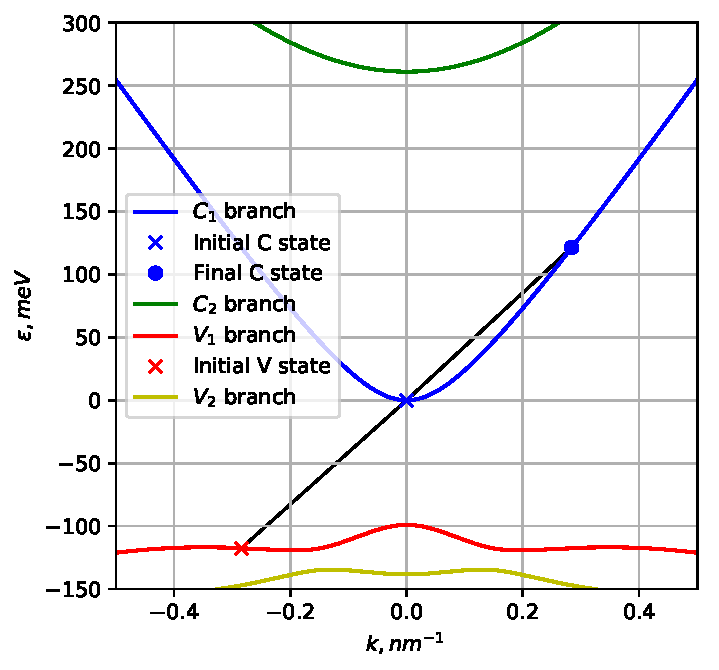
\includegraphics[width=1.\linewidth]{./images/main_14u_80K_pic.pdf}

                    \textbf{Рис. а: Образец с "грязными" КЯ.} Пороговая энергия 
                        $\varepsilon_{th} \approx 18.6~meV$.
                \end{center}
            \end{minipage}
            \hfill
            \begin{minipage}[h]{0.49\linewidth}
                \begin{center}
                    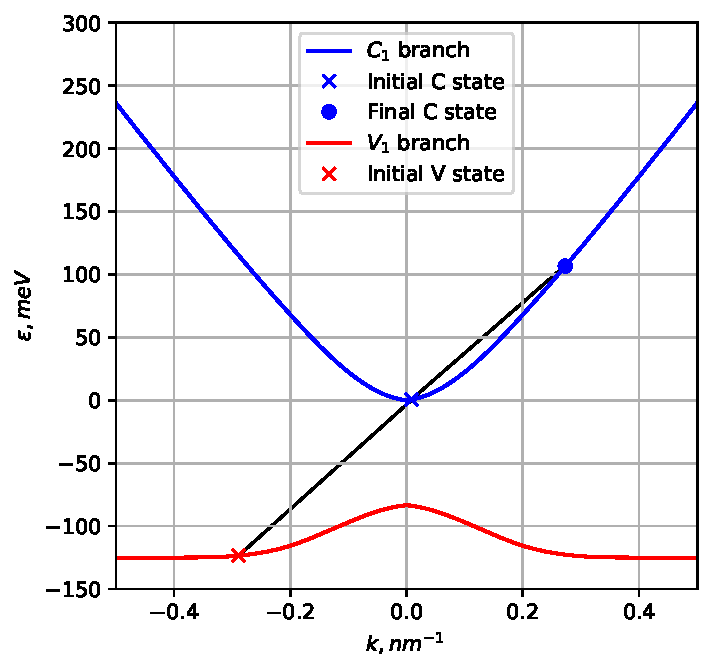
\includegraphics[width=1.\linewidth]{./images/14u_pure_80K.pdf}

                    \textbf{Рис. б: Образец с "чистыми" КЯ.} Пороговая энергия 
                        $\varepsilon_{th} \approx 23.3~meV$.
                \end{center}
            \end{minipage}
        \end{figure}
        
        Аналогично поступим и со структурой расчитаной для излучения на длине волны  
        $18~\mu m$. Результаты расчётов спектра электронов и дырок для двух случаев приведены на рисунке ниже. В первом случае (рис. а) расчёт проведён 
        для экспериментально исследованной Cd${}_{0.1}$Hg${}_{0.9}$Te/Cd${}_{0.65}$Hg${}_{0.35}$Te КЯ толщиной 8.7 nm, во втором случае (рис. б) расчёт проведён для 
        HgTe/Cd${}_{0.65}$Hg${}_{0.35}$Te КЯ толщиной 4.4 nm.
        
        \begin{figure}[h!]
            \begin{minipage}[h]{0.49\linewidth}
                \begin{center}
                    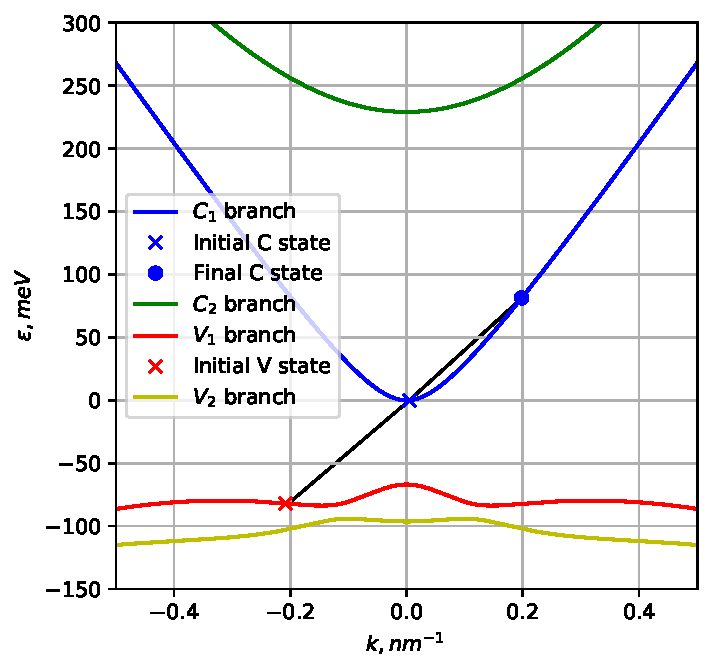
\includegraphics[width=1.\linewidth]{./images/18u_impure_40K.pdf}
    
                    \textbf{Рис. а: Образец с "грязными" КЯ.} Пороговая энергия 
                        $\varepsilon_{th} \approx 15~meV$.
                \end{center}
            \end{minipage}
            \hfill
            \begin{minipage}[h]{0.49\linewidth}
                \begin{center}
                    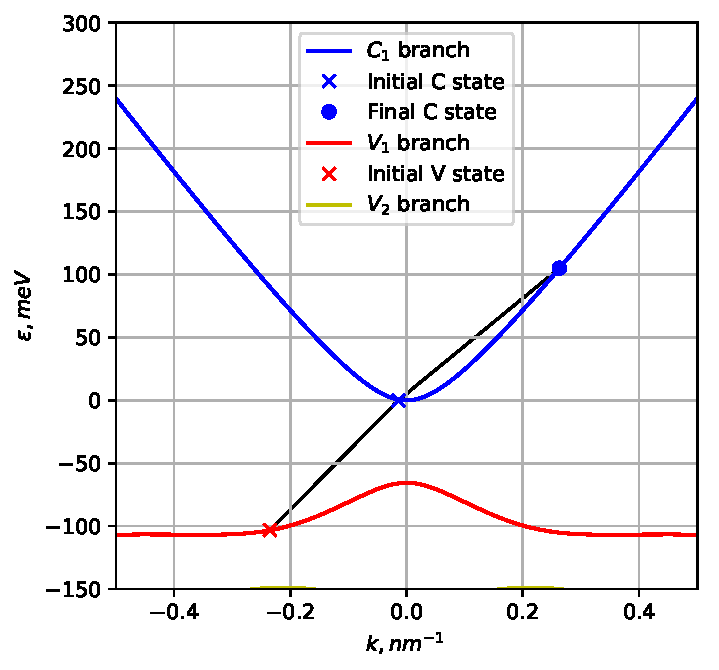
\includegraphics[width=1.\linewidth]{./images/18u_pure_40K.pdf}
    
                    \textbf{Рис. б: Образец с "чистыми" КЯ.} Пороговая энергия 
                        $\varepsilon_{th} \approx 37.3~meV$.
                \end{center}
            \end{minipage}
        \end{figure}

        Из рисунка a видно, что для первого случая в валентных подзонах имеются дополнительные максимумы, располагающиеся ниже потолка валентной 
        зоны на 7 meV. В HgTe яме, окруженной Cd${}_{0.65}$Hg${}_{0.35}$Te, эти экстремумы практически отсутствуют (рис. б). Как было показано ниже
        вид дисперсионного соотношения может существенно влиять на порог оже-процессов.
        \newpage

        \section{Зависимость оже-порога в зависимости от состава барьера}

        Рассмотрим влияние высоты барьеров на порог оже-процессов. Для 
        этого рассмотрим подробнее структуру для излучения на длине волны $18~\mu m$,
        в силу большего интереса к длиноволновому стимулированному излучению.

        Интересно сравнить пороговые энергии для структуры, описанной выше, и структур на основе квантовых ям HgTe. На рисунке ниже представлена 
        зависимость пороговой энергии оже-рекомбинации (вычисленной в модели) и толщины КЯ при двух разных концентрациях состава ям
        от доли Cd в барьерах для температуры 40K, 
        при фиксированной величине ширины запрещённой зоны, составляющей $67~meV$. Из рисунка видно, что максимальная пороговая энергия (что оптимально 
        с точки зрения максимальной температуры генерации стимулированного излучения) достигает величины 38 meV при доле Cd 0.67 и чистой яме, а также 
        17 meV при высоте барьеров в 0.3.

    \begin{figure}[h]
    \vspace{0.75cm}
    \begin{minipage}[h]{\linewidth}
        \begin{center}
            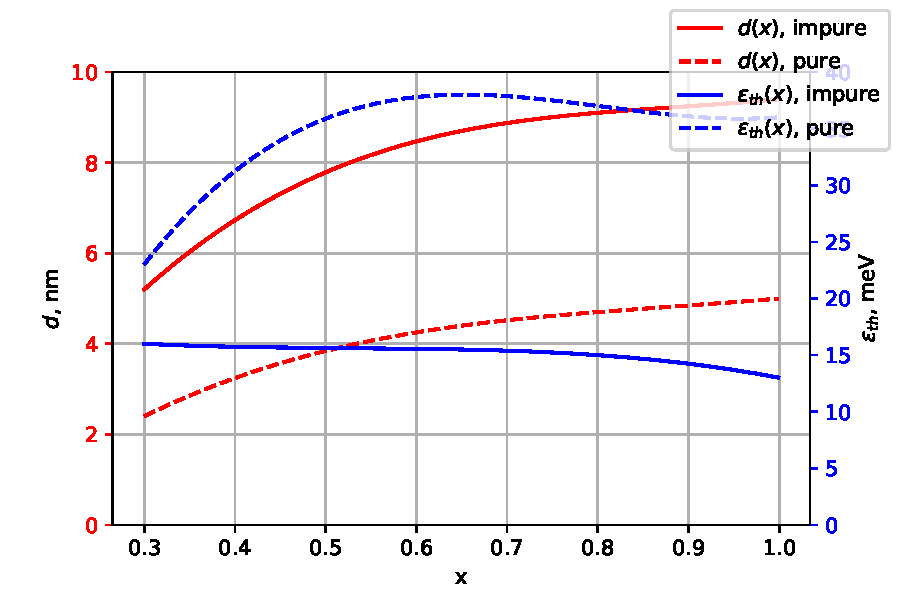
\includegraphics[width=1\linewidth]{./images/de_vs_x.pdf}

            \vspace{0.75cm}
            \textbf{Пороговая энергия Оже-процессов и толщина КЯ.}
            Расчеты проводились при $T= 40~K$, $E_g \approx 67~meV$.
            \vspace{1.25cm}
        \end{center}
    \end{minipage}
    \end{figure}

    Из сравнения начальных состояний частиц для случаев с "чистой" и "грязной" ямой в предыдущем разделе видно, 
    что «эффективная масса» дырок для оже-процесса в HgTe квантовой яме 
    существенно меньше, чем в Cd${}_{0.1}$Hg${}_{0.9}$Te квантовой яме. Это связано с наличием в в Cd${}_{0.1}$Hg${}_{0.9}$Te квантовой яме ярко выраженного бокового 
    экстремума в верхней валентной подзоне. Хорошо известно, что увеличение эффективной массы дырок приводит к снижению пороговой энергии 
    Оже-процесса. Наличие максимума на зависимости пороговой энергии от доли кадмия в HgTe/Cd${}_{x}$Hg${}_{1-x}$Te обусловлено наличием минимума 
    «эффективной массы» дырок при определенной доле кадмия. Следует отметить, условность использованного здесь термина «эффективная масса» 
    для верхней валентной подзоны, поскольку закон дисперсии в ней не квадратичный и, вообще говоря, немонотонный.

    Таким образом, было продемонстрировано, что при заданной энергии межзонного перехода пороговая энергия оже-рекомбинации в структурах 
    HgTe/Cd${}_{x}$Hg${}_{1-x}$Te с КЯ является немонотонной функцией от доли кадмия в барьере. При оптимальной концентрации кадмия в барьерах и КЯ из HgTe 
    можно ожидать почти двухкратного повышения критической температуры стимулированного излучения по сравнению с прототипной структурой с 
    Cd${}_{0.1}$Hg${}_{0.9}$Te/Cd${}_{0.65}$Hg${}_{0.35}$Te КЯ.

    \section{Перспективные структуры}

    В данном случае нас больше всего интересует связь между возникновением побочных максимумов и некоторым количеством 
    кадмия, который оказывается напыленным внутри квантовых ям. Очевидно, что использование более чистых в этом смысле структур
    может предотвратить возникновение канала оже-рекомбинации типа CCHC через них. Однако кроме того методом численной оптимизации параметров 
    подобных структур могут быть получены параметры, при которых порог оже-рекомбинации в теории будет являться бесконечным (в частности можно добиться почти 
    гиперболического закона дисперсии). Однако на текущий момент подобные структуры не могут быть выращены в силу высоких требований к чистоте исполнения и 
    прецизионного выдерживания толщины КЯ. Более того в таких случаях невозможно рассмотрение лишь радиальной составляющей дисперсионного соотношения,
    поскольку учёт зависимости $\varepsilon(\varphi)$ будет всегда давать более низкий порог Оже-рекомбинации.

    Более того, наличие подобных боковых минимумов превращает подобную структуру в квазинепрямозонную, что может радикально снижать возможность излучательной 
    рекомбинации из этих точек k-пространства. 

    Также в качестве осложняющего обстоятельства нельзя не упомянуть существенное различие концентрации кадмия в квантовых ямах в плоскости структуры,
    что, с одной стороны, обуславливает возможность изучения образцов с одинаковой структурой, с другой - плохо влияет на воспроизводимость измерений,
    а также осложняет сравнение полученных результатов с теорией.

    Возможно, перспективным будет являться создание структур с легированием, что позволит искусственно повысить одного из типов носителей заряда и реализовать 
    ситуацию в которой, вопреки дисперсионному соотношению будет превалировать тот или иной механизм Оже-рекомбинации. Это может быть полезным как с точки зрения 
    фундаментальных исследований, так и с точки зрения простоты оптимизации структур (можно будет заботиться о темпе рекомбинации всего по одному механизму). 
    Более того это может интересно в перспективе с позиции создания быстрых полупроводниковых детектеров, работающих в этой же области электромагнитного спектра 
    (в данном случае оже-процессы будут играть уже положительную роль).
\end{document}